\section{Versuchsprogramm und Übersicht}
\label{sec:versuchsprogramm}

Mit den Rädern aus PA46-GF30 wurden zehn Laufversuche auf dem Prüfstand KV3 gefahren, der Vorversuch zur Temperatur aus \secref{sec:temperatur} und neun Wöhlerversuche auf den Stufen $8$, $12$ und $16$\,Nm am Rad mit zwei, drei und vier Rädern. Alle Läufe sind beendet, ein Durchläufer liegt nicht vor. Die Drehzahl betrug $3058$\,1/min am Ritzel, also $3000$\,1/min am Rad, die Öltemperatur an der Messstelle vor der Prüfverzahnung $74$ bis $75$\,\textdegree C und in den Läufen bei $16$\,Nm $67$\,\textdegree C. Der Prüfstand hält bei einem Abfall des Moments um $1$\,Nm an. Bei jedem Halt wurde nachgespannt, wobei das Moment um höchstens $5$\,\% über dem Sollwert eingestellt wurde. Ab dem Lauf mit dem Rad 97360 wurden bei jedem Halt die markierten Zähne fotografiert. \figref{fig:risswachstum_97364} zeigt diese Dokumentation am Rad 97364 bei $8$\,Nm, dem am längsten gelaufenen Rad, als Ausschnitt gleicher Größe um die markierten Zähne. Die Reihe deckt das Anrissfenster zwischen $3{,}65$ und $6{,}61 \cdot 10^{6}$ Lastwechseln und das Risswachstum bis zum Ende des Laufs ab, bei dem kein Zahn brach. Die früheren Läufe tragen schriftliche Befunde zum Zustand der Fußrundungen. \tabref{tab:versuchsprogramm_pa46} nennt je Rad die Stufe, die Öltemperatur und die Lastwechselzahl am Ende. Dazu kommen die versagten Zähne nach der Sichtprüfung der gelaufenen Räder (\secref{sec:schadensbilder}), das wirksame Kriterium nach \secref{sec:auswertung_laufversuche} und der Zählerstand der ersten sichtbaren Anrisse. Die Lastwechselzahlen sind die Zählerstände der Ritzelwelle aus der Arbeitsmappe des Prüfstands nach \secref{sec:auswertung_laufversuche}.

\begin{figure}[!htbp]
	\centering
	\begin{subfigure}[t]{0.30\textwidth}
		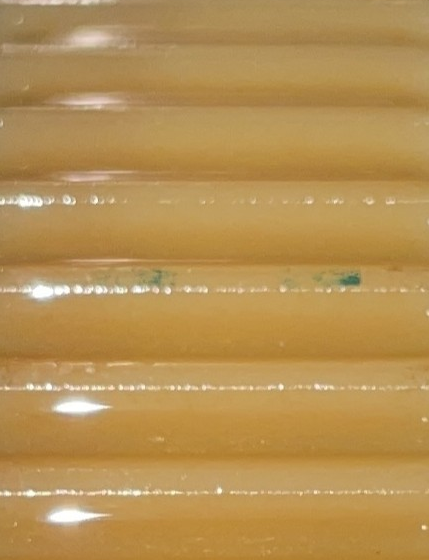
\includegraphics[width=\textwidth]{kap6/risswachstum_97364_3653000}
		\caption{$3{,}65 \cdot 10^{6}$}
	\end{subfigure}\hfill
	\begin{subfigure}[t]{0.30\textwidth}
		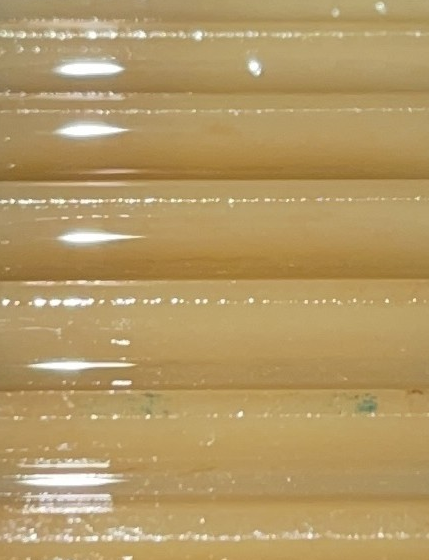
\includegraphics[width=\textwidth]{kap6/risswachstum_97364_6610000}
		\caption{$6{,}61 \cdot 10^{6}$}
	\end{subfigure}\hfill
	\begin{subfigure}[t]{0.30\textwidth}
		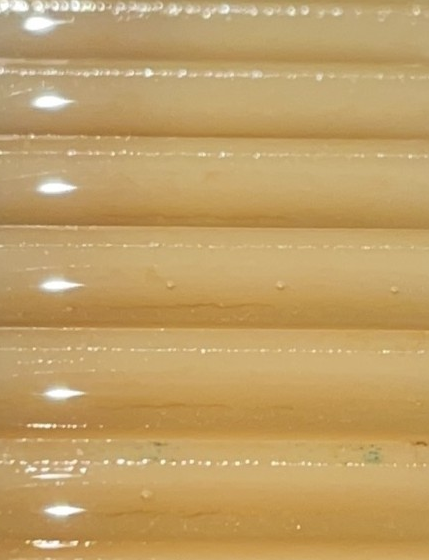
\includegraphics[width=\textwidth]{kap6/risswachstum_97364_8410000}
		\caption{$8{,}41 \cdot 10^{6}$}
	\end{subfigure}\\[4pt]
	\begin{subfigure}[t]{0.30\textwidth}
		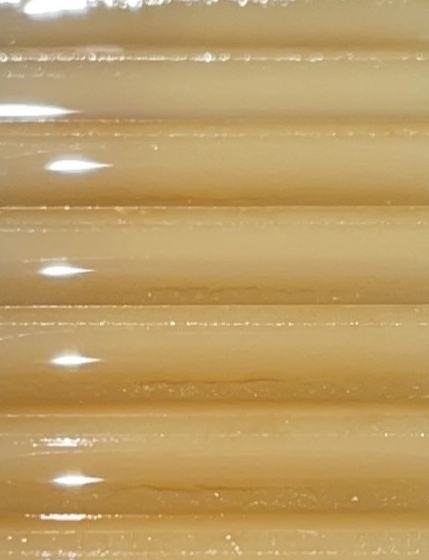
\includegraphics[width=\textwidth]{kap6/risswachstum_97364_11161000}
		\caption{$11{,}16 \cdot 10^{6}$}
	\end{subfigure}\hfill
	\begin{subfigure}[t]{0.30\textwidth}
		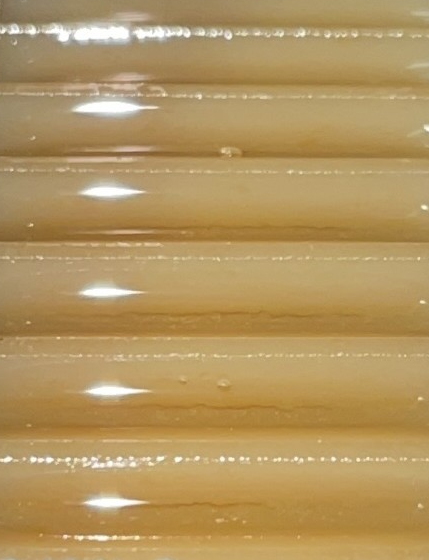
\includegraphics[width=\textwidth]{kap6/risswachstum_97364_14810000}
		\caption{$14{,}81 \cdot 10^{6}$}
	\end{subfigure}\hfill
	\begin{subfigure}[t]{0.30\textwidth}
		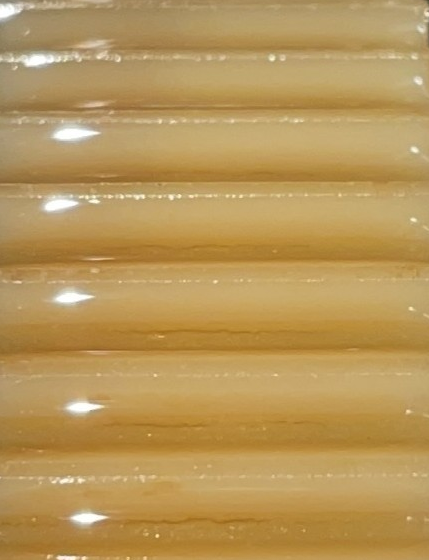
\includegraphics[width=\textwidth]{kap6/risswachstum_97364_18365000}
		\caption{$18{,}37 \cdot 10^{6}$}
	\end{subfigure}\\[4pt]
	\begin{subfigure}[t]{0.30\textwidth}
		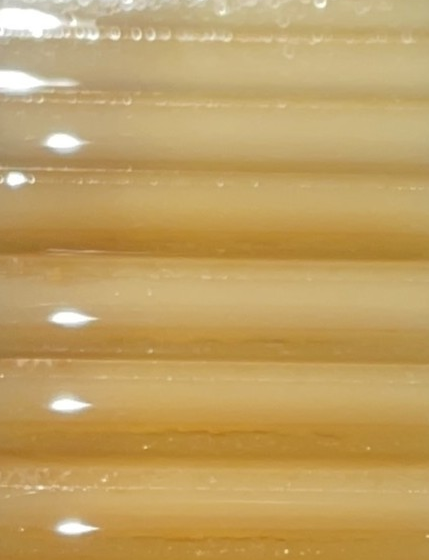
\includegraphics[width=\textwidth]{kap6/risswachstum_97364_23770000}
		\caption{$23{,}77 \cdot 10^{6}$}
	\end{subfigure}\hfill
	\begin{subfigure}[t]{0.30\textwidth}
		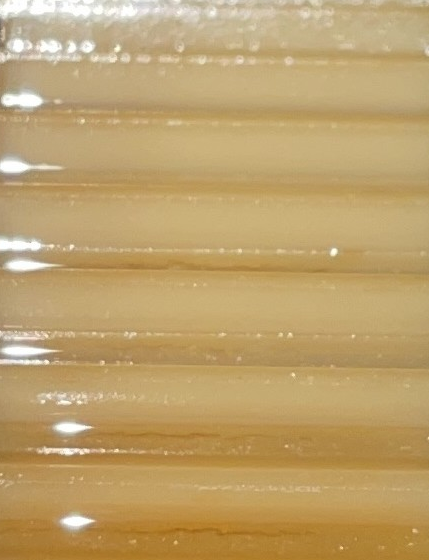
\includegraphics[width=\textwidth]{kap6/risswachstum_97364_32015000}
		\caption{$32{,}02 \cdot 10^{6}$}
	\end{subfigure}\hfill
	\begin{subfigure}[t]{0.30\textwidth}
		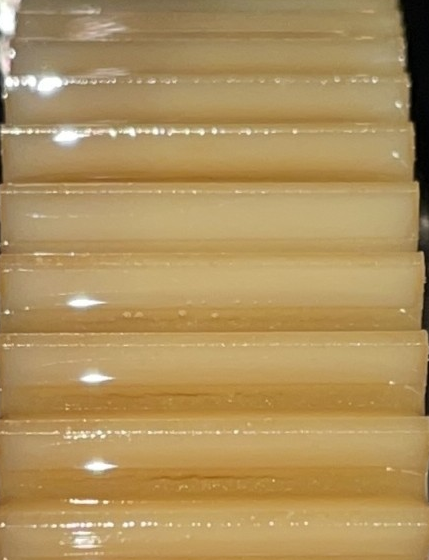
\includegraphics[width=\textwidth]{kap6/risswachstum_97364_40000000}
		\caption{$40 \cdot 10^{6}$ (geschätzt)}
	\end{subfigure}
	\caption{Rad 97364 bei $8$\,Nm, markierte Zähne bei jedem Halt des Prüfstands, Ausschnitt gleicher Größe um die Markierung (links die belastete Flanke mit dem Zahnfuß): keine Anrisse bei $3{,}65 \cdot 10^{6}$, leichte Haarrisse bei $6{,}61 \cdot 10^{6}$, Anrisse einzeln sichtbar ab $8{,}41 \cdot 10^{6}$, deutlich sichtbar ab $14{,}81 \cdot 10^{6}$ Lastwechseln, Ende beim lauten Versagensgeräusch ohne vollständigen Zahnfußbruch.}
	\label{fig:risswachstum_97364}
\end{figure}

\begin{table}[htbp]
	\caption{Laufversuche mit PA46-GF30 auf dem Prüfstand KV3 im Jahr 2026: ME-Nummer des Rades, Stufe des Raddrehmoments, Öltemperatur an der Messstelle, Lastwechselzahl am Ende, versagte Zähne nach der Sichtprüfung, wirksames Kriterium und erste sichtbare Anrisse (spätestens ab: erste Kontrolle mit Befund, zwischen: letzte Kontrolle ohne und erste Kontrolle mit Befund).}
	\label{tab:versuchsprogramm_pa46}
	\centering
	\footnotesize
	\setlength{\tabcolsep}{4pt}
	\begin{tabular}{L{1.3cm}L{0.8cm}L{0.8cm}L{1.9cm}L{2.5cm}L{1.7cm}L{2.2cm}L{2.4cm}}
		ME-Nummer & $T_{2}$ in Nm & Öl in \textdegree C & Lastwechsel                 & versagte Zähne                                                & Kriterium           & erste Anrisse                               & Vermerk                                                   \\
		\hline
		\arrayrulecolor{black!30}
		97351     & $12$          & $75$                & $2{,}42 \cdot 10^{6}$       & 34 bis 41 abgebrochen                                         & Totalausfall        & keine bis $2{,}20 \cdot 10^{6}$             & Stufenlauf nach der Temperaturmatrix                      \\
		\hline
		97350     & $12$          & $74$                & $6{,}21 \cdot 10^{6}$       & 37 bis 41 abgebrochen                                         & Totalausfall        & nicht dokumentiert                          & Ende nicht im Protokoll notiert                           \\
		\hline
		97365     & $12$          & $74$                & $3{,}78 \cdot 10^{6}$       & 41 abgebrochen; 39, 40 und 44 bis 47 angerissen               & Totalausfall        & nicht dokumentiert                          &                                                           \\
		\hline
		97345     & $8$           & $74$                & $24{,}96 \cdot 10^{6}$      & 34 abgebrochen                                                & Totalausfall        & zwischen $3{,}22$ und $7{,}66 \cdot 10^{6}$ & erste $1{,}25 \cdot 10^{6}$ Lastwechsel bei etwa $10$\,Nm \\
		\hline
		97346     & $16$          & $67$                & $1{,}51 \cdot 10^{6}$       & 40, 41 abgebrochen; 38, 39 angerissen                         & Totalausfall        & spätestens ab $1{,}40 \cdot 10^{6}$         &                                                           \\
		\hline
		97366     & $16$          & $67$                & $1{,}21 \cdot 10^{6}$       & 31, 32 abgebrochen; 38 bis 40 Fußbruch; 37 Flankenbruch       & Totalausfall        & spätestens ab $0{,}96 \cdot 10^{6}$         & abrasiver Verschleiß vor dem Bruch                        \\
		\hline
		97355     & $16$          & $67$                & $1{,}37 \cdot 10^{6}$       & 39, 40 abgebrochen; 38 Flankenbruch                           & Totalausfall        & spätestens ab $0{,}95 \cdot 10^{6}$         & Verschleiß vor dem Bruch                                  \\
		\hline
		97340     & $16$          & $67$                & $1{,}92 \cdot 10^{6}$       & 36 bis 38 Fußbruch; 39, 40 Flankenbruch; 28 bis 31 angerissen & Totalausfall        & spätestens ab $1{,}72 \cdot 10^{6}$         & Anrisse an allen Zähnen                                   \\
		\hline
		97360     & $12$          & $74$                & $4{,}57 \cdot 10^{6}$       & 38 bis 41 angebrochen                                         & Totalausfall        & spätestens ab $2{,}53 \cdot 10^{6}$         & Bilder je Halt                                            \\
		\hline
		97364     & $8$           & $75$                & $40 \cdot 10^{6}$ geschätzt & kein Bruch                                                    & Versagens\-geräusch & zwischen $3{,}65$ und $6{,}61 \cdot 10^{6}$ & Drehzahlsensor ausgefallen                                \\
		\hline
		\arrayrulecolor{black}
	\end{tabular}
\end{table}

% TK erledigt (Zähne nach der Liste des Nutzers vom 2026-10-21 eingetragen, Anrissspalte mit "spätestens ab" und "zwischen", Spalte Lauf gestrichen): Tim liefert noch die genauen Zähne nach, die abgebrochen sind. Aber die Tabelle enthält eine merkwürdige Aufschlüsselung der Anrisse. das bis deutet hin, bis dahin schadensfrei, aber das würde ich umformulieren. Also nicht bis ohne und dann in allen anderen Zeilen nur noch bis, sondern eher ab

Beim Rad 97345 war das Moment nach dem Start versehentlich auf etwa $10$\,Nm am Rad eingestellt und wurde beim ersten Halt nach $1{,}25 \cdot 10^{6}$ Lastwechseln auf die Stufe gesetzt. Der Punkt wird mit diesem Vermerk geführt. Beim Rad 97364 fiel der Drehzahlsensor nach $32 \cdot 10^{6}$ Lastwechseln aus. Die Endzahl von $40 \cdot 10^{6}$ ist aus der Laufzeit nach dem letzten bekannten Zählerstand geschätzt. Der Lauf wurde beim lauten Versagensgeräusch beendet, bevor ein Zahn brach. Die abgebrochenen und angebrochenen Zähne liegen bei sieben der neun gebrochenen Räder vollständig zwischen den Zähnen 31 und 41, also in einem Fünftel des Umfangs von 52 Zähnen. Außerhalb liegen nur die Anrisse der Zähne 28 bis 31 am Rad 97340 und 44 bis 47 am Rad 97365. An drei Rädern der Stufe $16$\,Nm liegt der Bruch einzelner Zähne nicht im Fuß, sondern in der Flanke über der Spur der Ritzelkopfkante (\secref{sec:schadensbilder}).

Als Vergleich dienen die 14 Laufversuche mit POM auf derselben Verzahnung aus dem Jahr 2023, die Fiederling auf dem Prüfstand KV4 bei $2250$\,1/min am Rad und $73$ bis $76$\,\textdegree C Öltemperatur ausgewertet hat \cite[S.~43 und 65]{Fie23}. Dort sind die Stufen nach dem Ritzelmoment benannt, so dass die Stufe $16$\,Nm am Rad $16{,}3$\,Nm trägt. Die Bilder und Tabellen dieser Arbeit führen das Raddrehmoment. Außerhalb bleiben nach \secref{sec:pruefstand} die Läufe des Jahres 2023 mit $45$\,\textdegree C Öltemperatur, die Stufenläufe, die Läufe bei anderen Drehzahlen und alle Läufe mit PEEK.

Zwei Beobachtungen am Prüfstand gehören zur Übersicht. Erstens schwankte das angezeigte Moment bei $2250$\,1/min auch bei frischer Verzahnung deutlich, bei $3000$\,1/min dagegen nicht. Ein größeres Flankenspiel oder eine Zahnverformung scheidet bei frischer Verzahnung als Ursache aus. Als Ursachen kommen das Mittelungsfenster der Anzeige, eine Faltung der umlaufperiodischen Anteile durch die Abtastung der Steuerung oder eine Torsionsresonanz des Verspannungskreises nahe einer Harmonischen von $37{,}5$\,Hz in Frage. In das Mittelungsfenster passen bei $3000$\,1/min ganze Radumdrehungen von $20$\,ms, bei $2250$\,1/min mit $26{,}7$\,ms nicht. Die Messwelle erfasst das Moment mit Dehnmessstreifen und gibt ein Analogsignal an die Steuerung \cite[S.~52]{Schu09}. Eine Abtastrate ist in der Quelle nicht genannt. Zweitens ist die Nachspannhistorie eine Überlagerung aus Verschleiß, Kriechen, Zahnbiegung und Rissen, weil jeder Weg im Verspannungskreis das Moment senkt. \tabref{tab:verlustraten_97364} zeigt das am Beispiel des Rades 97364, des am längsten gelaufenen und am dichtesten protokollierten Rades. Der Momentverlust je Intervall zwischen zwei Halten fällt nach dem Einlauf von $5{,}5$ auf $0{,}2$\,Nm je $10^{6}$ Lastwechsel, während die Anrisse ab $8{,}4 \cdot 10^{6}$ Lastwechseln einzeln und ab $14{,}8 \cdot 10^{6}$ deutlich sichtbar wurden. Bei diesem Rad treiben die Risse den Momentverlust nicht. Die Rate folgt eher der Aggregattemperatur, die zwischen $8$ und $15 \cdot 10^{6}$ Lastwechseln $91$ bis $93$\,\textdegree C erreichte. Für die übrigen Räder liegen die Halte zu weit auseinander, um die Rate so aufzulösen. Eine Prüfanweisung für die weiteren Läufe folgt in \chapref{chap:zusammenfassung}.

% TK erledigt (Beobachtungen neu: Schwankung als Beobachtung, Nachspannhistorie nur als Beispiel 97364): Der Abschnitt ist mehr oder weniger falsch dargestellt. Bitte nochmal mit meinen Anmerkungen gegenprüfen, die ich jetzt über den gesametn Text verteitl habe und wenn dir nichts auffält, dann an mich fragen, Aber der Abschnitt ist nicht ordentlich und korrekt formuliert. Und Tabelle 6 ist jetzt einfach verwendet, da ich da sehr viel protokolliert habe, aber das sollte dann auch exemplarisch verwednet werden und nicht als pauschale textfeststellung so übernommen werden, dass das eine generelle Aussage der Raten ist.

\begin{table}[htbp]
	\caption{Momentverlust je Nachspannintervall am Rad 97364 ($8$\,Nm) als Beispiel: Verlust aus dem Protokoll, Rate je $10^{6}$ Lastwechsel, Temperatur des Aggregats $\vartheta_{\mathrm{A}}$ und der Messstelle vor der Prüfverzahnung $\vartheta_{\mathrm{P}}$.}
	\label{tab:verlustraten_97364}
	\centering
	\footnotesize
	\begin{tabular}{L{2.4cm}L{2.4cm}L{2.0cm}L{2.8cm}L{1.7cm}L{1.7cm}}
		von                    & bis                    & Verlust in Nm & Nm je $10^{6}$ Lastwechsel & $\vartheta_{\mathrm{A}}$ in \textdegree C & $\vartheta_{\mathrm{P}}$ in \textdegree C \\
		\hline
		\arrayrulecolor{black!30}
		$0{,}05 \cdot 10^{6}$  & $0{,}27 \cdot 10^{6}$  & $1{,}2$       & $5{,}45$                   & $80$                                      & $75$                                      \\
		\hline
		$0{,}27 \cdot 10^{6}$  & $3{,}65 \cdot 10^{6}$  & $1{,}0$       & $0{,}30$                   & $83$                                      & $75$                                      \\
		\hline
		$3{,}65 \cdot 10^{6}$  & $6{,}61 \cdot 10^{6}$  & $1{,}0$       & $0{,}34$                   & $86$                                      & $76$                                      \\
		\hline
		$6{,}61 \cdot 10^{6}$  & $8{,}41 \cdot 10^{6}$  & $1{,}7$       & $0{,}94$                   & $91$                                      & $77$                                      \\
		\hline
		$8{,}41 \cdot 10^{6}$  & $11{,}16 \cdot 10^{6}$ & $1{,}8$       & $0{,}65$                   & $93$                                      & $77$                                      \\
		\hline
		$11{,}16 \cdot 10^{6}$ & $14{,}81 \cdot 10^{6}$ & $1{,}4$       & $0{,}38$                   & $93$                                      & $77$                                      \\
		\hline
		$14{,}81 \cdot 10^{6}$ & $18{,}37 \cdot 10^{6}$ & $1{,}2$       & $0{,}34$                   & $83$                                      & $75$                                      \\
		\hline
		$18{,}37 \cdot 10^{6}$ & $23{,}77 \cdot 10^{6}$ & $1{,}7$       & $0{,}31$                   & $84$                                      & $75$                                      \\
		\hline
		$23{,}77 \cdot 10^{6}$ & $32{,}02 \cdot 10^{6}$ & $1{,}6$       & $0{,}19$                   & $81$                                      & $75$                                      \\
		\hline
		\arrayrulecolor{black}
	\end{tabular}
\end{table}

% Herkunft:
% Absatz 1 (Programm, Regeln): 80_output/messungen/laufversuche/laufversuche.md (Tabelle PA46-GF30, KV3 2026) aus
%   kst-E_Laufversuche_KV3.xlsx Zeilen 77 bis 95; Regeln: Spalte U Zeile 94 (kst-E_74: "nach 1 Nm Drehmomentabfall
%   nachverspannt mit max +5 % Drehmomentabweichung vom Sollmoment", Abbruchkriterium Loss of drive, 1 Nm über
%   100 000 LW), Nutzer 2026-10-18 (Startmoment über der Stufe, damit das Sollmoment in der Mitte liegt; Bilder
%   der markierten Zähne ab kst-E_74; keine Durchläufer; 3058 = Ritzel, 3000 = Rad; Öl = Messstelle);
%   ADR-118 Amendment 2026-10-18 Abend Punkt 1, 4, 5. Messwelle: SA-1272.txt Druckseite 52 (4.7.3).
% Tabelle: laufversuche.md und anrissfenster.md (Anriss: 69 3 223 000 bis 7 658 000; 75 3 653 000 bis 6 610 000;
%   74 ≤ 2 530 000; 70 ≤ 1 404 000; 71 ≤ 962 000; 72 ≤ 945 000; 73 ≤ 1 719 000; 63 "keine Auffälligkeit" bei
%   2 198 207); Zähne: Spalte J (34; 40 und 41; 31; 39; 40); Vermerke: test_runs_user.yaml (Nutzer 2026-10-18).
% Absatz 2 (69, 75, Zähne): Spalte T Zeile 89 (1251000 9,6 Nm, "falsches Drehmoment eingestellt"), Spalte M 10,3 Nm
%   am Ritzel = 10,5 am Rad; Zeile 95 (Drehzahlsensor ausgefallen bei 32 015 000, Schätzung 40 000 000, "sehr
%   laut", "noch keine Zähne locker"); Fenster 36 bis 40: parts.yaml failure_window, kap3_3 und kap4_4.
% Absatz 3 (Vergleich): 80_output/messungen/woehler/vergleich.md (POM KV3 n = 6: 53, 54, 55, 56, 57, 67; PEEK KV3
%   n = 6: 58 bis 62, 64; POM KV4 n = 14; PEEK KV4 n = 12; ausgeschlossen 65, 29 ohne Drehzahl, 32/34 4000, 33/35
%   1000, 39 3000 1/min); laufversuche.md (kst-E_1 bis 7 Öl 45 °C, kst-E_22 Stufenlauf, 50 bis 52 Trockenlauf RT);
%   Stufenbenennung 2023 nach Ritzelmoment: Spalte K gegen Q (16 → 16,3136); MA-0296 = Fie23.
% Absatz 4 (Beobachtungen): Nutzer 2026-10-18 (Schwankung bei 2250 1/min bei frischer Verzahnung; Nachspannhistorie
%   als Überlagerung); Hypothesen: Antwort vom 2026-10-18 (ADR-118 Amendment Abend Punkt 5); SA-1272.txt
%   Druckseite 52 (DMS, Analogsignal, keine Abtastrate); 80_output/messungen/laufversuche/verlustraten.md
%   (kst-E_75: 5,45/0,30/0,34/0,94/0,65/0,38/0,34/0,31/0,19 Nm je Mio., TA 80 bis 93, TP 74 bis 77);
%   Anrisse: Spalte T Zeile 95 (8410000 "Anrisse einzeln sichtbar", 14810000 "deutlich sichtbar").
% Bild fig:risswachstum_97364 (2026-10-25): neun Fotos des Nutzers je Halt (Dateiname = Lastwechsel), Befunde aus
%   Spalte T Zeile 95 der Arbeitsmappe (3653000 keine Anrisse; 6610000 leichte Haarrisse; 8410000 Anrisse einzeln
%   sichtbar; 11161000 keine große Veränderung; 14810000 deutlich sichtbar; 18365000, 23770000, 32015000 deutlich
%   sichtbar, Versagensgeräusch ab 27160000; 40000000 geschätzt, Ende sehr laut, keine Zähne locker).
%   2026-10-25 Abend: die Rohfotos 11161000 und 14810000 waren beim Beschriften vertauscht und wurden vom Nutzer
%   benannt zurückgetauscht (Umbenennung in 70_input); Ausschnitt des letzten Fotos unter dem Ritzel (WINDOW_TOP).
% Bibwunsch: Fie23, Schu09 vorhanden.
% Nomenklatur: vartheta_A, °C, Temperatur des Ölaggregats (Mappe "TA"); vartheta_P, °C, Öltemperatur an der
%   Messstelle vor der Prüfverzahnung (Mappe "TP"); T_2 vorhanden.
% Offen: Welle des Lastwechselzählers; Fenster 36 bis 40; PEEK-Typ; Zitierweise der Versuche 2026; die
%   Prüfanweisung steht in Kapitel 8 (noch nicht entworfen).
